

\subsection{Ordinary least square, Ridge, and Lasso regression with resampling on the Franke function}

In this subsection we will present Ordinary least square, Ridge and Lasso regression up to the fifth order, with a resampling technic, k-fold, on the Franke function. The Mean square error, (MSE), $R^2$ score function and the confidence intervall is also presented. 

%Presenter OLS analyse av Frank funksjonen, med polynomial fit - $[x, y, x^2, y^2, xy].$ Ta med kyss-validering og k-sampling. etter dette; samme operasjon men med Ridge og Lasso regression. med bias $(\lambda)$.

\subsubsection{Ordinary least square}
Here we present the OLS regression with up to a fifth order polynomial fit on Franke function, notice that in the plot we use a fifth order polynomial, the $R^2$ score and MSE according to order of the polynomial used for fitting of the data. And lastly a table containing the $\beta$ values, the variance, and the confidence intervall according to the different polynomials

The confidence intervall of $\beta$ through variance. The mean squared error(MSE) and the $R^2$ score function. 
Presenting the resampling of the data, where the data have been splitt into training and test data. 
Implementing k-folding and reevaluates MSE, $R^2$, on the test data. Finding Bias and variance with $Err(x_0) = irreducible Error + Bias^2 + variance$



\begin{figure}[H]
\centering
      \begin{subfigure}{0.45\textwidth}
       	\centering
       	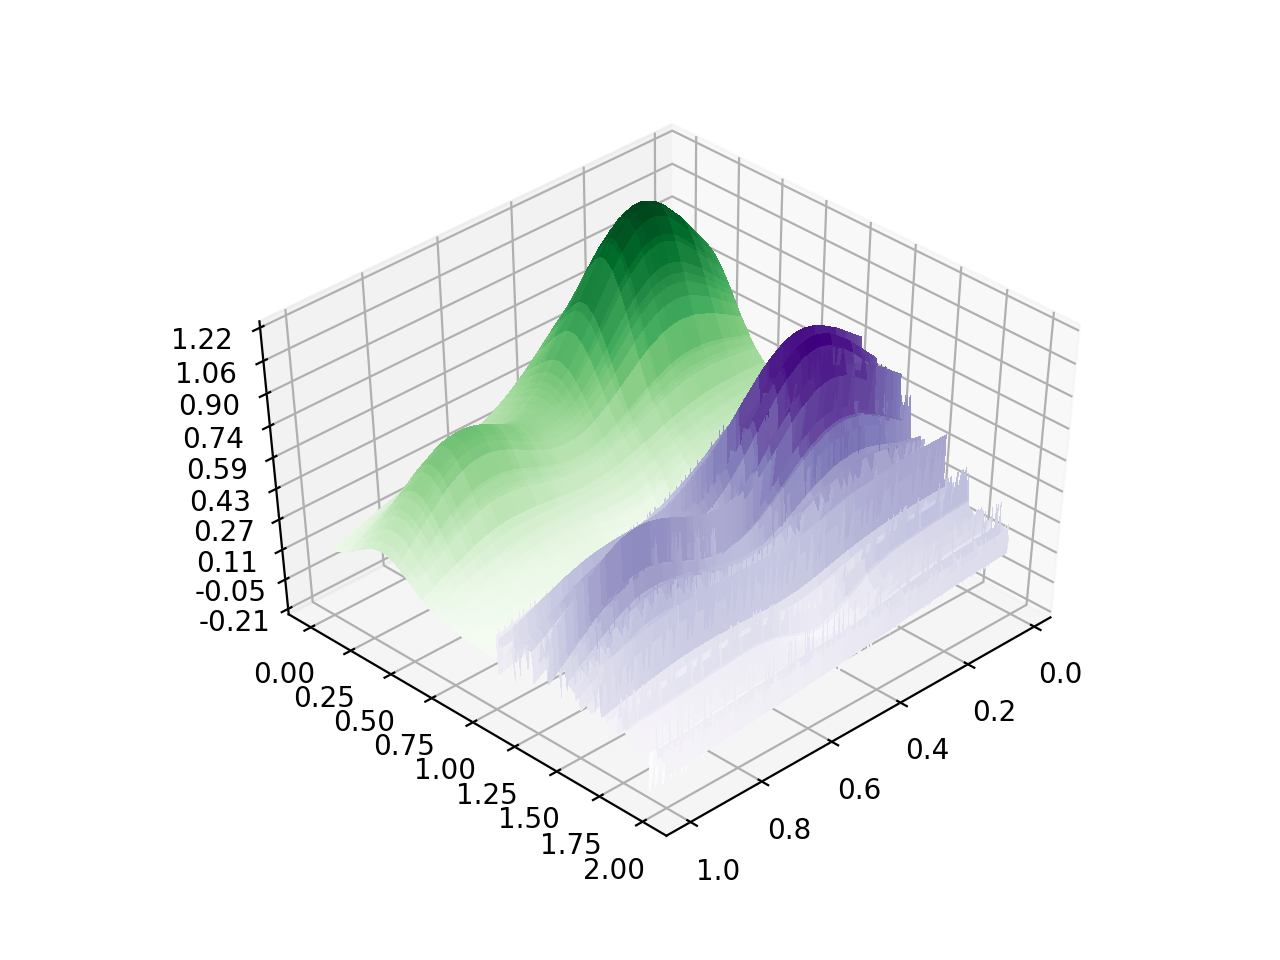
\includegraphics[width=\linewidth]{result/bilder/Franke_noise.png}
        	\caption{}
     \end{subfigure}
     ~
     \begin{subfigure}{0.45\textwidth}
       	\centering
       	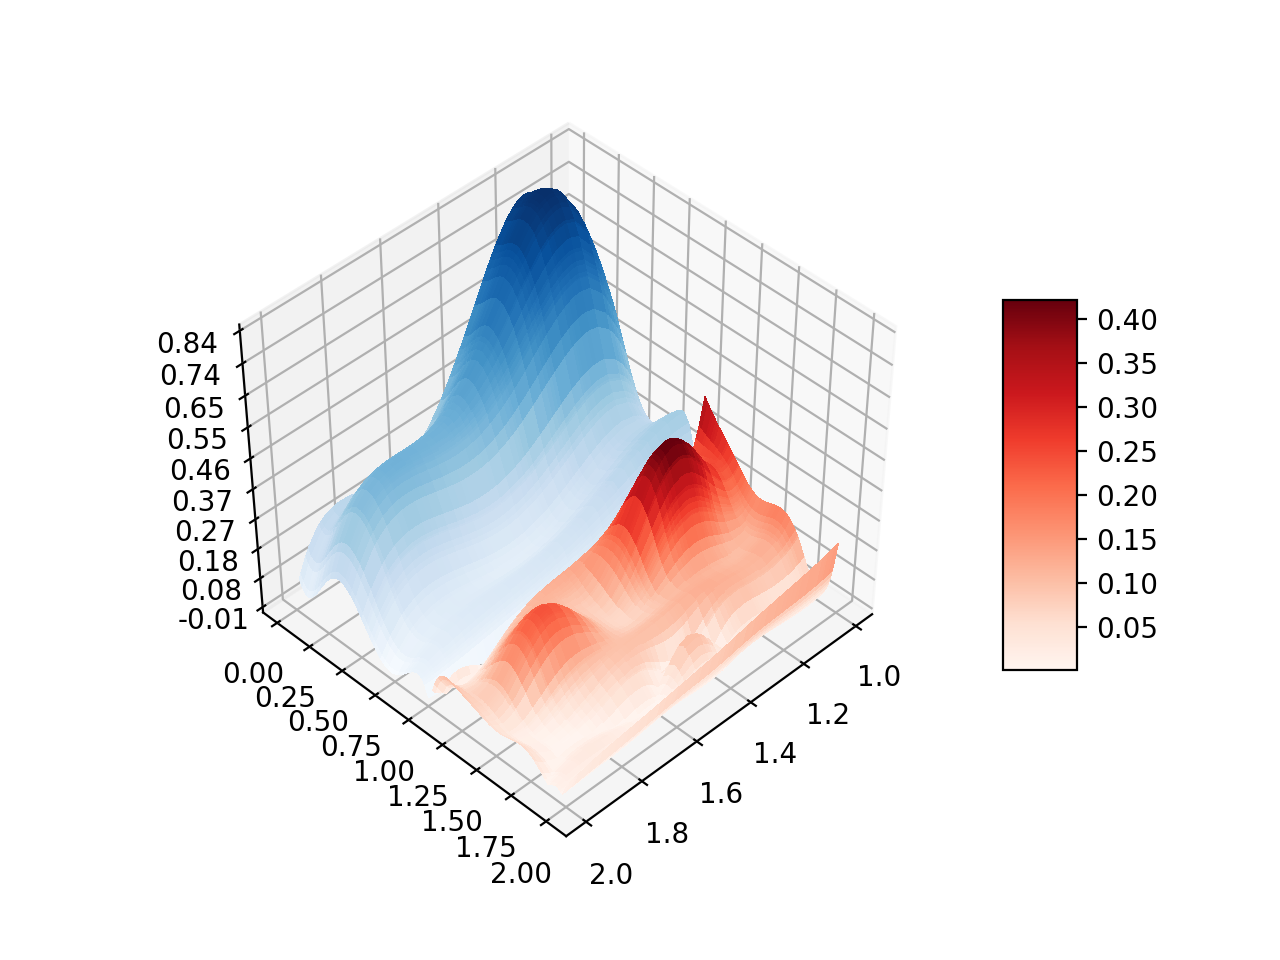
\includegraphics[width=\linewidth]{result/bilder/OLS_bar.png}
        	\caption{}
    	\end{subfigure}
 	\caption{a) Franke function plottet in green, and the Frank function with noise plottet in purple. b) Our fifth order approximation of the Franke function plottet in blue. On the right we have the residuals, i.e. the error compared to the real function, and its relative size indicated by the red colour gradient.}
	\label{fig:OLS_Frank}
\end{figure}


 \begin{center}
 \label{tab:OLS_Degree_R2_MSE}
 \captionof{table}{MSE and $R^2$ score for OLS by degree. These values are created by taking the average values over 100 different executions, with a noise level $= 0.1$ and a $\lambda/\alpha = 0.00001$ }
 \begin{tabularx}{\textwidth}{c X c X c  }
     \hline
     \hline
         Degree && R2 && MSE \\
         \hline
2      && 0.71 && 0.01353 \\ 
3      && 0.81 && 0.00916 \\ 
4      && 0.86 && 0.00712 \\ 
5      && 0.88 && 0.00585 \\ \hline
 \end{tabularx}
 \end{center}
 
  \begin{center}
 \label{tab:Confidenceintervall_OLS}
 \captionof{table}{$\beta$, Var and Confidence intervall for OLS by degree of $x$ and $y$. }
 \begin{tabularx}{\textwidth}{c X l X l X l }
     \hline
     \hline
     $x^iy^j$ && $\beta$ && VAR && Confidence intervall \\
     \hline
$x^0y^0$     && 0.259   && 0.001   &&  [0.227, 0.291]     \\ 
$x^0y^1$     && 4.117   && 0.108   &&  [3.788, 4.446]     \\ 
$x^0y^2$     && -18.065 && 2.943   &&  [-19.781, -16.349] \\ 
$x^0y^3$     && 29.764  && 15.934  &&  [25.772, 33.756]   \\ 
$x^0y^4$     && -22.199 && 17.571  &&  [-26.391, -18.007] \\ 
$x^0y^5$     && 6.361   && 2.637   &&  [4.737, 7.985]     \\ 
$x^1y^0$     && 5.277   && 0.074   &&  [5.005, 5.549]     \\ 
$x^1y^1$     && -9.751  && 1.234   &&  [-10.862, -8.64]   \\ 
$x^1y^2$     && 13.591  && 6.186   &&  [11.104, 16.078]   \\ 
$x^1y^3$     && -21.609 && 7.858   &&  [-24.412, -18.806] \\ 
$x^1y^4$     && 12.635  && 1.628   &&  [11.359, 13.911]   \\ 
$x^2y^0$     && -22.726 && 1.825   &&  [-24.077, -21.375] \\ 
$x^2y^1$     && 28.964  && 5.900   &&  [26.535, 31.393]   \\ 
$x^2y^2$     && -1.849  && 6.149   &&  [-4.329, 0.631]    \\ 
$x^2y^3$     && -5.401  && 1.364   &&  [-6.569, -4.233]   \\ 
$x^3y^0$     && 30.056  && 10.123  &&  [26.874, 33.238]   \\ 
$x^3y^1$     && -36.035 && 7.072   &&  [-38.694, -33.376] \\ 
$x^3y^2$     && 6.742   && 1.441   &&  [5.542, 7.942]     \\ 
$x^4y^0$     && -11.919 && 12.008  &&  [-15.384, -8.454]  \\ 
$x^4y^1$     && 12.813  && 1.444   &&  [11.611, 14.015]   \\ 
$x^5y^0$     && -0.909  && 1.951   &&  [-2.306, 0.488]    \\ 

     \hline
 \end{tabularx}
 \end{center}

 
\subsubsection{Ridge regression}
Samme analyse ( samme polynomiales og resampling teknikk) med forskjellige verdier av lambda. % *SAMMENLIGN MED DATA FRA TIDLIGRE* 
Se på avhengigheten av lambda imens du varierer mengden bråk(noise i Franke).
 
 \begin{center}
 \label{tab:Ridge_Degree_R2_MSE}
 \captionof{table}{MSE and $R^2$ score for Ridge by degree. These values are created by taking the average values over 100 different executions, with a noise level $= 0.1$ and a $\lambda = 0.00001$}
 \begin{tabularx}{\textwidth}{c X c X c  }
     \hline
     \hline
         Degree && R2 && MSE \\
         \hline
2      && 0.71 && 0.01353 \\ 
3      && 0.80 && 0.00968 \\ 
4      && 0.81 && 0.00928 \\ 
5      && 0.81 && 0.00902 \\ \hline
 \end{tabularx}
 \end{center}
 
\begin{center}
 \label{tab:OLS_lambda_R2_MSE}
 \captionof{table}{ MSE and $R^2$ score for OLS by degree. These values are created by taking the average values over 100 different executions, with a noise level $= 0.1$}
 \begin{tabularx}{\textwidth}{c X c X c  }
     \hline
     \hline
         $\lambda/\alpha$ && R2 && MSE \\
         \hline
 0.0000001  && 0.81150  && 0.00587 \\
0.0000100  && 0.80979  && 0.00605 \\
0.0010000  && 0.74059  && 0.00592 \\
0.1000000  && -0.20901 && 0.00608 \\
1.0000000  && -1.85170 && 0.00613 \\
2.0000000  && -1.83823 && 0.00586 \\
5.0000000  && -1.79681 && 0.00601 \\
10.0000000 && -1.81950 && 0.00591\\ \hline
 \end{tabularx}
 \end{center}


  \begin{center}
 \label{tab:Confidenceintervall_Ridge}
 \captionof{table}{$\beta$, Var and Confidence intervall for Ridge by degree of $x$ and $y$. }
 \begin{tabularx}{\textwidth}{c X c X c X c }
     \hline
     \hline
     $x^iy^j$ && value && variance && confidence intervall \\
     \hline
$x^0y^0$     && 0.384    && 0.001   && x \\
$x^0y^1$     && 1.770    && 0.077   && x \\
$x^0y^2$     && -0.294   && 1.953   && x \\
$x^0y^3$     && -22.690  && 10.474  && x \\
$x^0y^4$     && 41.542   && 12.033  && x \\
$x^0y^5$     && -20.675  && 1.949   && x \\
$x^1y^0$     && 5.348    && 0.068   && x \\
$x^1y^1$     && -11.544  && 1.040   && x \\
$x^1y^2$     && 18.567   && 4.891   && x \\
$x^1y^3$     && -27.573  && 6.071   && x \\
$x^1y^4$     && 14.943   && 1.295   && x \\
$x^2y^0$     && -21.987  && 1.712   && x \\
$x^2y^1$     && 32.153   && 5.221   && x \\
$x^2y^2$     && -5.093   && 5.179   && x \\
$x^2y^3$     && -3.142   && 1.161   && x \\
$x^3y^0$     && 25.775   && 9.426   && x \\
$x^3y^1$     && -39.259  && 6.976   && x \\
$x^3y^2$     && 6.673    && 1.214   && x \\
$x^4y^0$     && -4.833   && 11.244  && x \\
$x^4y^1$     && 14.552   && 1.590   && x \\
$x^5y^0$     && -4.681   && 1.908   && x \\ 
    \hline
 \end{tabularx}
 \end{center}
 

\subsubsection{Lasso regression}
Presenter det samme igjen, men med Lasso regression  på Frank, Vurder de tre metodene opp mot hverandre 


 \begin{center}
 \label{tab:Lasso_Degree_R2_MSE}
 \captionof{table}{MSE and $R^2$ score for Lasso by degree. These values are created by taking the average values over 100 different executions, with a noise level $= 0.1$ and a $\lambda/\alpha = 0.00001$}
 \begin{tabularx}{\textwidth}{c X c X c  }
     \hline
     \hline
         Degree && R2 && MSE \\
         \hline
2      && 0.71 && 0.01353 \\ 
3      && 0.81 && 0.00916 \\ 
4      && 0.86 && 0.00712 \\ 
5      && 0.88 && 0.00585 \\ \hline
 \end{tabularx}
 \end{center}
 
 
 \begin{center}
 \label{tab:Degree_R2_MSE}
 \captionof{table}{MSE and $R^2$ score for Lasso on Franke function by $\lambda$. These values are created by taking the average values over 100 different executions, with a noise level $= 0.1$}
 \begin{tabularx}{\textwidth}{c X c X c  }
     \hline
     \hline
$\lambda$    &&R2     &&MSE     \\
         \hline
0.0000001 &&0.87497&&0.00587 \\
0.0000100 &&0.87517&&0.00605 \\
0.0010000 &&0.87723&&0.00592 \\
0.1000000 &&0.87242&&0.00608 \\
1.0000000 &&0.87708&&0.00613 \\
2.0000000 &&0.87833&&0.00586 \\
5.0000000 &&0.87572&&0.00601 \\
10.0000000 && 0.87528&&0.00591
 \end{tabularx}
 \end{center}
 
\subsection{Ordinary least square, Ridge, and Lasso regression with resampling, now on real data}

\begin{figure}[H]
		\centering
		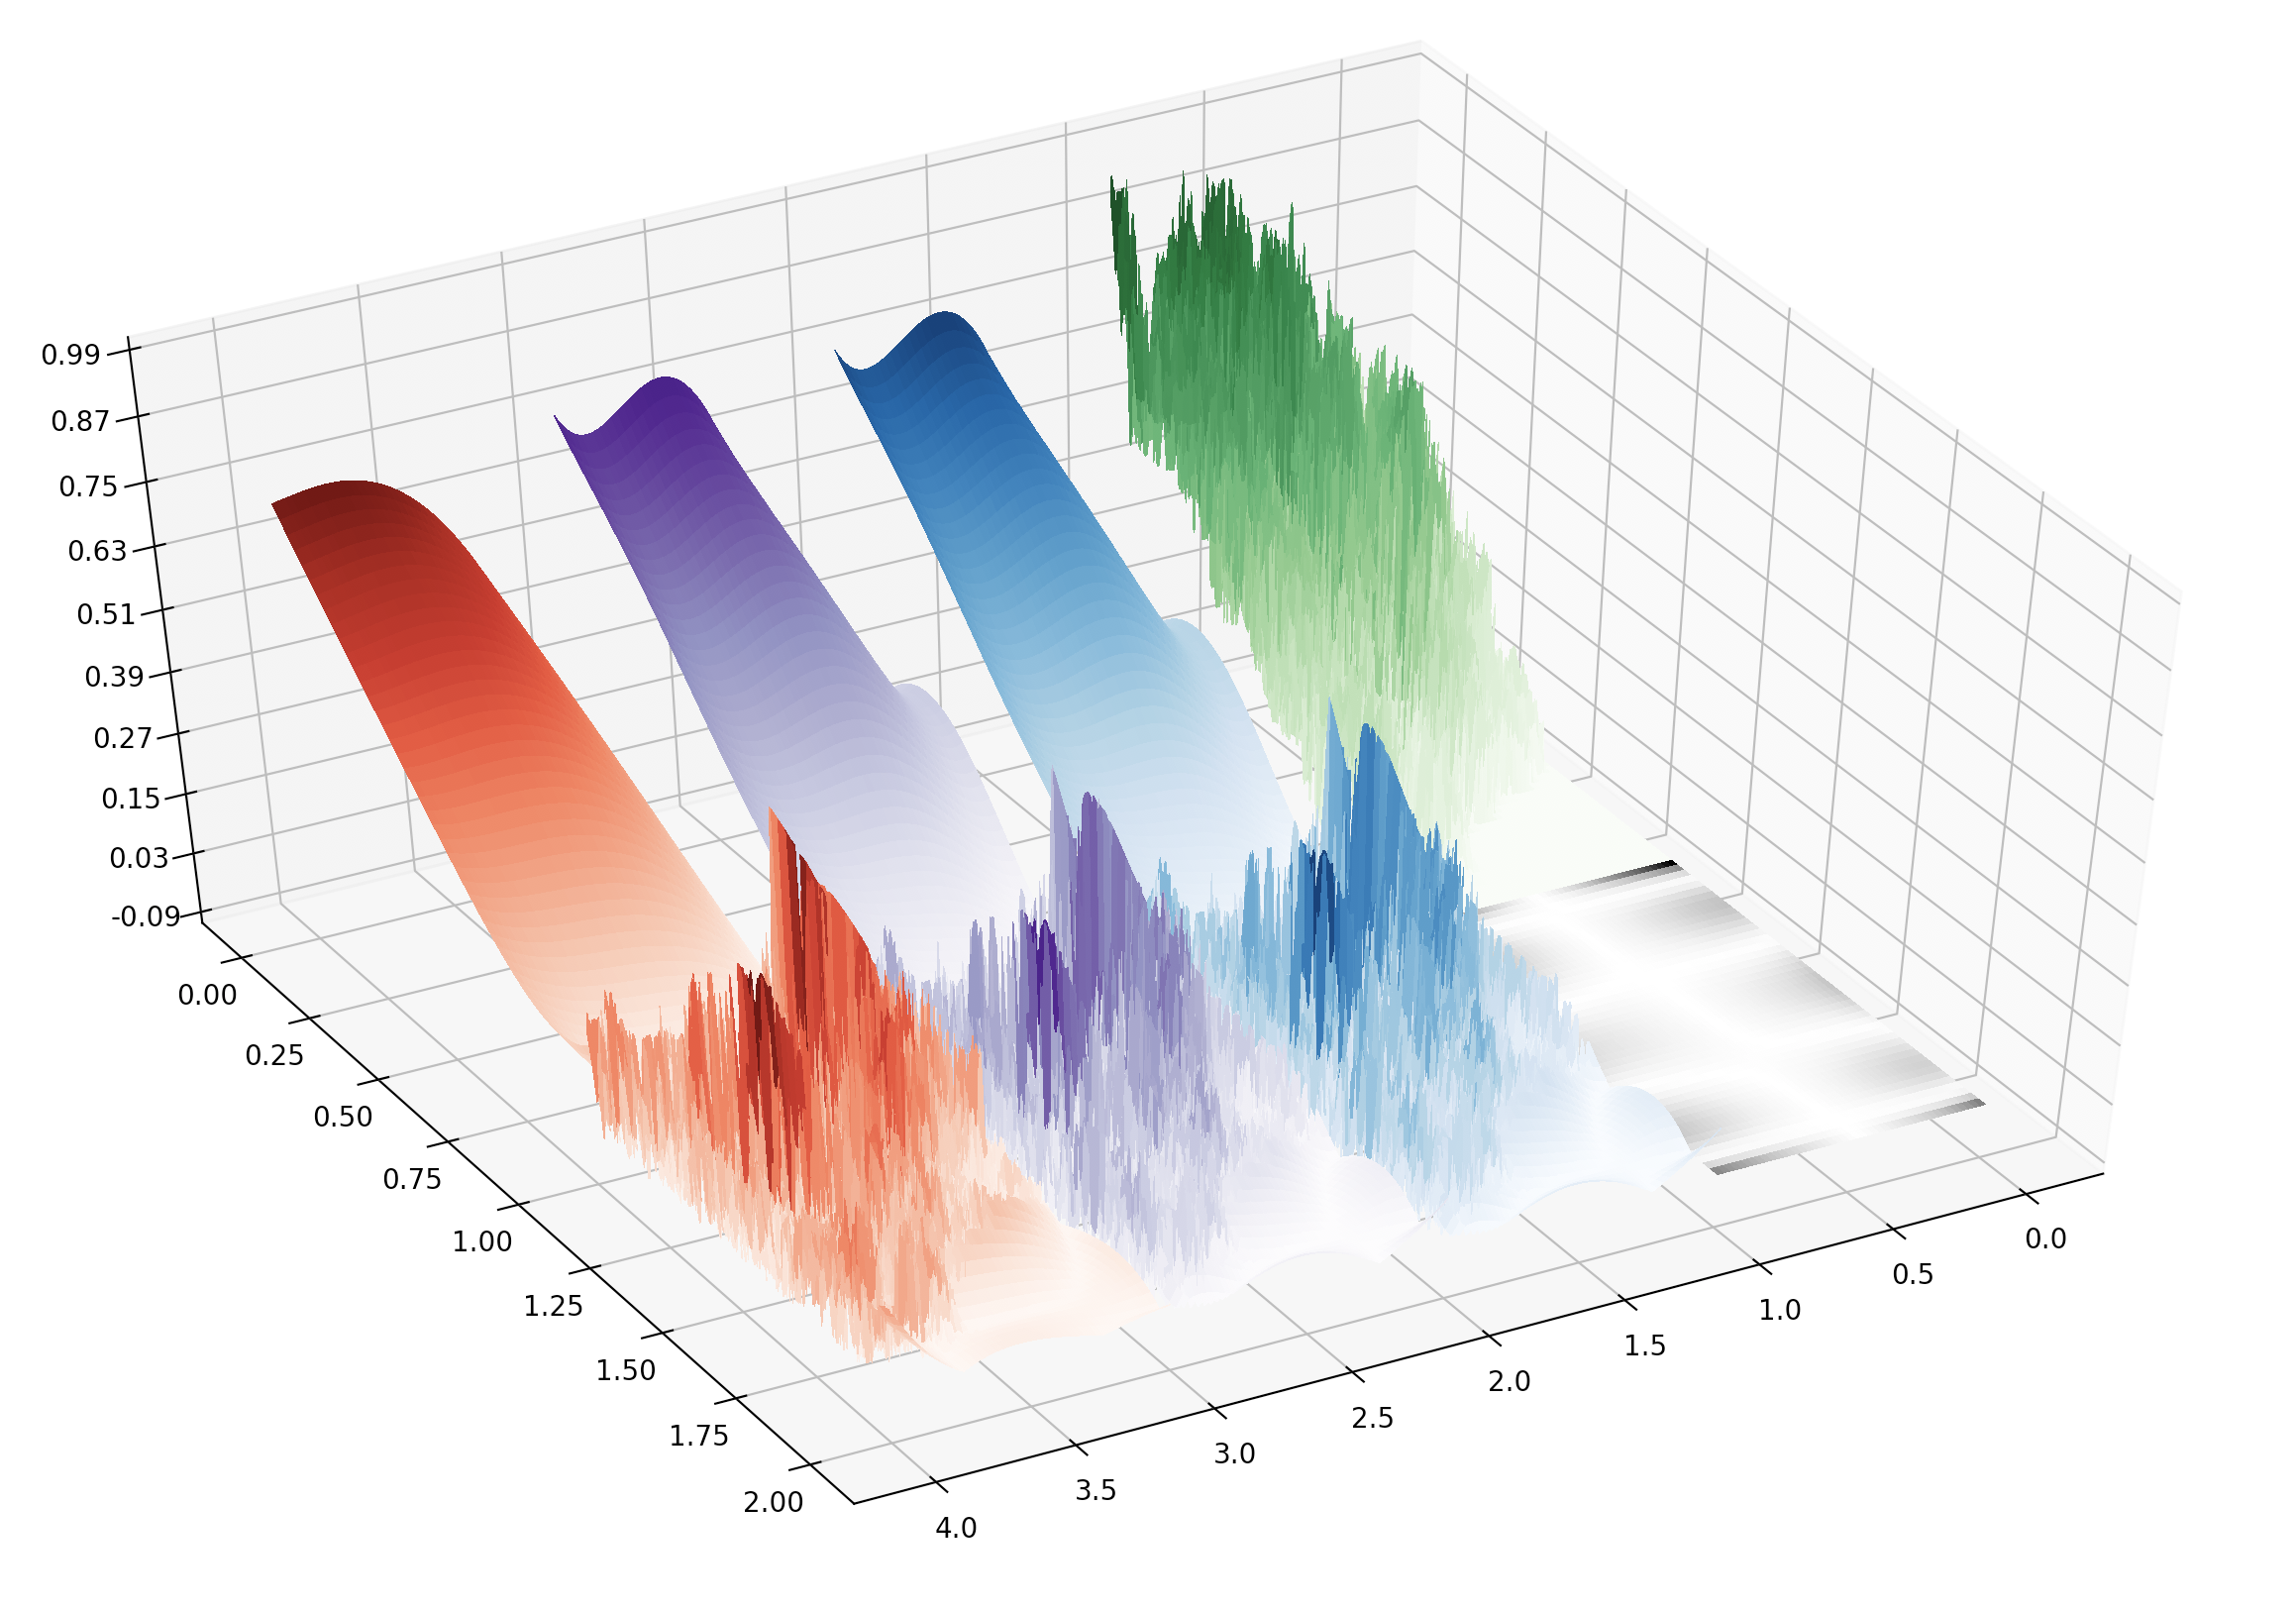
\includegraphics[width=1.1\linewidth]{result/bilder/all_real.png}
		\caption{REAL DATAAAA.}
		\label{fig:RealData}
\end{figure}


 \begin{center}
 \label{tab:Realdata_OLS_lambda_R2_MSE}
 \captionof{table}{OLS on realdata. Can see that $R^2$ "går til helvete", when big alpha, so no point in plotting for higher alpha }
 \begin{tabularx}{\textwidth}{c X c X c  }
     \hline
     \hline
$\lambda$    &&R2     &&MSE     \\
         \hline
0.0000001 && 0.823088 && 0.010720 \\
0.0000100 && 0.823088 && 0.010720 \\
0.0010000 && 0.823088 && 0.010720 \\
0.1000000 && 0.823088 && 0.010720 \\
 \end{tabularx}
 \end{center}

 \begin{center}
 \label{tab:Realdata_Lasso_lambda_R2_MSE}
 \captionof{table}{Lasso on realdata. We saw that $R^2$ got out of hand with a $\lambda = 0.1$ and higher, and decided not to include those numbers. }
 \begin{tabularx}{\textwidth}{c X c X c  }
     \hline
     \hline
$\lambda$    &&R2     &&MSE     \\
         \hline
0.0000001 && 0.797486 && 0.012272 \\
0.0000100 && 0.797470 && 0.012273 \\
0.0010000 && 0.753280 && 0.014950 \\
0.1000000 && -0.165026 && 0.070596 \\
 \end{tabularx}
 \end{center}

 \begin{center}
 \label{tab:Realdata_Ridge_lambda_R2_MSE}
 \captionof{table}{Ridge on realdata. MSE and $R^2$ score for Ridge on the real data by $\lambda$. }
 \begin{tabularx}{\textwidth}{c X c X c  }
     \hline
     \hline
$\lambda$    &&R2     &&MSE     \\
         \hline
0.0000001 && 0.823088 && 0.010720 \\
0.0000100 && 0.823088 && 0.010720 \\
0.0010000 && 0.823027 && 0.010724 \\
0.1000000 && 0.818116 && 0.011022 \\
 \end{tabularx}
 \end{center}





%Presenter en kristisk vurdering og diskuter applikasjonsmulighetene(applicability) av disse regresjonsmetodene til typen data som blir presentert her. DISKUSJONSDEL

